\documentclass[12pt]{exam}
\newcommand{\hwnumber}{9}
\newcommand{\hwname}{Generic Queues}
\newcommand{\duedate}{\formatdate{8}{04}{\YEAR} by \progDueTime}

\usepackage{../misc/latex/edition}  % Course semester
\usepackage{../misc/latex/c0}       % Listings style for c0
\usepackage{amsmath}
\usepackage{enumerate}
\usepackage[normalem]{ulem}
\usepackage{verbatim}
\usepackage[left=1in, right=1in, top=1in, bottom=1in]{geometry}
\usepackage{graphicx}
\usepackage{hyperref}
\usepackage{tikz}     \usetikzlibrary{shapes}
\usepackage{fancybox}
\usepackage[all]{xy}
\usepackage{wrapfig}
\usepackage{fancyvrb}
\usepackage{datetime}
\usepackage{etoolbox}
\usepackage{calc}
\usepackage[nomessages]{fp}
\usepackage{import}  % Like input and include, but respects subdirectories

\newcommand{\defaultQuestionLocation}{questions}
\newcommand{\inputQuestion}[2][\defaultQuestionLocation/]{%
  \subimport{#1}{#2}
}
% Subdirectories of \defaultQuestionLocation containing code and pictures
\newcommand{\code}{code}
\newcommand{\img}{img}


%%% ic: frontmatter macros
\newcommand{\specialInstructions}{}
\newcommand{\HWNUMBER}
{\ifdefempty{\hwnumber}{__}{%
  \ifnumless{\hwnumber}{10}{0\hwnumber}{\hwnumber}}}
\newcommand{\hwtype}{Written Homework}

%%% ic: 'exam' tweaks
\renewcommand{\half}{.5} % Half points

\newcommand{\Question}[2][]
 {\ifstrempty{#1}
    {\question{\bf #2}}
    {\question[#1]{\bf #2}}
  \immediate\write\rubricfile{}%
  \immediate\write\rubricfile{Question \thequestiontitle:}%
  \immediate\write\rubricfile{==========}
 }

%%% ic: Support for editable PDF
% counter name (some viewers misbehave if always the same)
\newcounter{editable}
\newcommand{\nextField}{\addtocounter{editable}{1}q\arabic{editable}}
\newcommand{\NextField}
 {\makebox[0pt][r]{\scalebox{0.1}{\color{White}\nextField}}}

% Color of edit area
\newcommand{\editAreaColor}{red}
% Single line answer:   \editableLine[extra parameters (optional)]{line width}
\newcommand{\editableLine}[2][]
{\textcolor{\editAreaColor}{%
 \underline{\hspace*{-0.25em}%
 \raisebox{-0.5ex}{%
 \TextField[width=#2, borderwidth=0, #1]{\NextField}}}}%
}
% Single line answer for code:  \editableLine[extra parameters (optional)]{line width}
\newcommand{\editableCodeLine}[2][]
{\textcolor{\editAreaColor}{%
 \underline{%
 \TextField[width=#2, height=1.5ex, borderwidth=0, #1]{\NextField}}}}
% Multiline answer:  \editableLine[extra parameters (optional)]{box height}
\newcommand{\editableBox}[2][]
{\leavevmode\hspace*{-0.1em}%
\TextField[height=#2, width=\linewidth,
           multiline=true, borderwidth=0.1, bordercolor=\editAreaColor,
           #1]{\NextField}}

%%%%% Same answer format as exams
\renewcommand{\rmdefault}{ppl}
\renewcommand{\sfdefault}{phv}
\newcommand{\answerColor}{Blue}

\ifprintanswers
\newcommand{\answer}[2]{\makebox[#1][c]{\color{\answerColor}#2}}
\else
\newcommand{\answer}[2]{\makebox[#1][c]{}\makebox[0pt]{\phantom{|}}}
\fi
\newcommand{\uanswer}[2]{\underline{\answer{#1}{#2}}}


%%% Write rubric snippet.  Usage:
% \RUBRIC
% any multi-line text (including \, #, %, whatever)
% ENDRUBRIC
%% (ENDRUBRIC should be on a line by itself)
\makeatletter
\def\RUBRIC
 {%
  \begingroup
  \let\do\@makeother\dospecials
  \endlinechar=`\^^J
  \@tofile%
 }
\def\ENDRUBRIC{ENDRUBRIC}
\def\@tofile#1^^J{%
  \def\@test{#1}%
  \ifx\@test\ENDRUBRIC
    \immediate\write\rubricfile{}  % End with an empty line
    \expandafter\@firstoftwo
  \else
    \expandafter\@secondoftwo
  \fi
  {\endgroup}%
  {\toks@{#1}%
   \begingroup\endlinechar=\m@ne
   \everyeof{\noexpand}%
   \xdef\@temp{\scantokens\expandafter{\the\toks@}}%
   \endgroup
   \immediate\write\rubricfile{\@temp}%
   \@tofile}%
}
\makeatother

%% Displays tags for an exercise in 'answer' mode
\newcommand{\TAGS}[1]
{\ifprintanswers%
  \rule{0em}{0ex}%
  \marginpar{\footnotesize%
    \fcolorbox{black}{Gray!25}{%
      \parbox[t]{2cm}{\raggedright\textbf{TAGS:}\\#1}}}%
  \ignorespaces%
 \fi}%


%% Page layout
\pagestyle{headandfoot}

\headrule
\header{\textbf{\courseNumber{} \hwtype{} \hwnumber}}
       {}
       {\textbf{Page \thepage\ of \numpages}}
\footrule
\footer{}{}{\COPYRIGHT}

\renewcommand{\partlabel}{\textbf{\thequestion.\thepartno}}
%\renewcommand{\partlabel}{\textbf{Task \thepartno}}
\renewcommand{\subpartlabel}{\textbf{\thesubpart.}}
\renewcommand{\thepartno}{\arabic{partno}}
\renewcommand{\thesubpart}{\alph{subpart}}
\pointpoints{pt}{pts}
\pointformat{\raisebox{0ex}[\height][0pt]{\fcolorbox{black}{yellow}{\themarginpoints}}}
\bonuspointformat{\raisebox{0ex}[\height][0pt]{\fcolorbox{black}{red}{\themarginpoints}}}
\marginpointname{\points}
\pointsinmargin
%\boxedpoints

\setlength\answerlinelength{2in}
\setlength\answerskip{0.3in}

\newcommand{\mkWrittenTitle}[1]{#1}
\newcommand{\mkDueDate}[1]{#1}
\newcommand{\mkEvalSummary}[1]{#1}
\newcommand{\mkGradetable}[1]{#1}



% This fixes an issue with the exam package version 2.6 and after,
% where 'framed' has been renamed to 'examframed' to avoid a conflict.
\ifcsmacro{examframed}{%
\newenvironment{framed}
{\begin{examframed}}
{\end{examframed}}
}{}

\begin{document}
\hwTitle

\noindent
For the programming portion of this week's homework, we'll explore a
slight variant on the \emph{queue} data structure discussed in
class. The challenge of this assignment is primarily adding new functionality
to generic queues and then translating this data structure into C.

\bigskip
\noindent
The code handout for this assignment is at
\begin{center}
\whereisthetgz{queues-handout.tgz}
\end{center}
The file \lstinline'README.txt' in the code handout goes over the
contents of the handout and explains how to hand the assignment in.
There is a EIGHT (8) HANDIN LIMIT.  We advise you to delay using most
of these submissions till the tasks in Section~\ref{sec:C1toC}, where
you will wrestle the C language for the first time.  Every additional
handin will incur a small (5\%) penalty (even if using a late day).


\section{A Different Implementation of Queues}

The function \lstinline'is_segment(start, end)' used for the queues
and stacks in the lecture notes was based on the idea of
inclusive/exclusive bounds: the data is stored in the list nodes from
\lstinline'start' (inclusive) to \lstinline'end' (exclusive).

In this assignment, we'll do things differently and implement queues
based on the idea of \emph{inclusive list segments}. Here is how we
define them:
\begin{itemize}
\item%
  If \lstinline'start' is \lstinline'NULL', then there is an inclusive
  list segment of length 0 from \lstinline'start' to \lstinline'end'
  (for any value of \lstinline'end', in other words, we don't care
  what \lstinline'end' is).
\item%
  If \lstinline'start' and \lstinline'end' are the same and
  \lstinline'start->next' is \lstinline'NULL', then there is an
  inclusive list segment of length 1 from \lstinline'start' to
  \lstinline'end'.
\item%
  If \lstinline'start' and \lstinline'end' are different and there is
  an inclusive list segment of length $n>0$ from
  \lstinline'start->next' to \lstinline'end', then there is an
  inclusive segment of length $n+1$ from \lstinline'start' to
  \lstinline'end'.
\end{itemize}

\subsection{Basic Queues (New Data Structure Invariant)}

A queue's header node \lstinline'Q' contains three fields,
\lstinline'front', \lstinline'back', and \lstinline'size', and it
represents a valid queue if there is an inclusive list segment of
length \lstinline'Q->size' from \lstinline'Q->front' to
\lstinline'Q->back'. This means the queues you will implement for this
assignment appear to take one of the two forms in
Figure~\ref{fig:datastruct}, depending on whether or not they are
empty.

\clearpage
\begin{figure}
\begin{center}
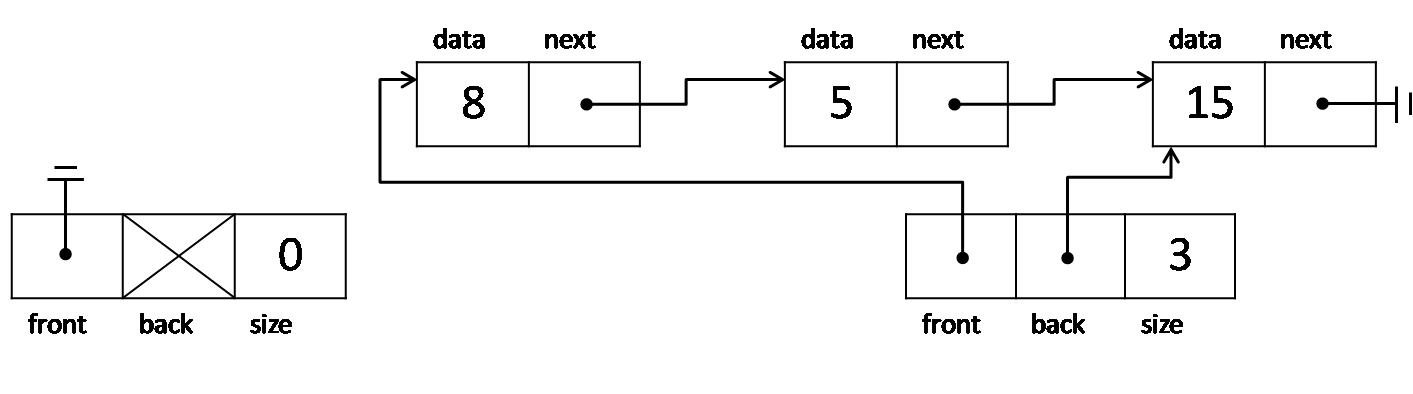
\includegraphics[width=0.9\linewidth]{img/queue.png}
\end{center}
\caption{Illustration of the data structure invariants for this assignment.}
\label{fig:datastruct}
\end{figure}

%% TODO S16: Actually make data fields pointers to ints.

Figure~\ref{fig:datastruct} is inaccurate in one way: our queues will
be \emph{generic}, so the \lstinline'data' field contains data of type
\lstinline'void*'. Therefore, the data field at the front of the
second queue could not actually contain the number 8. At best, it
could contain an \lstinline'int*', pointing to allocated memory
containing the number 8. Unlike other data structures like hash sets,
we \emph{do} allow the generic pointers in a queue to be
\lstinline'NULL'.

\begin{task}[2]
\TAGS{ds-invariant, genericity, linked-list, queue, void-star}
  In \lstinline'queue.c1', implement the specification function
  \lstinline'is_queue(Q)' according to the specification above.  You
  may find it simpler to write \lstinline'is_segment' recursively.
\end{task}

The basic interface for queues is mostly the same as the one in class,
extended to be generic by making the elements void pointers. Another
difference is that we expose a constant-time function that reports on
the size of the queue, since we're storing that information anyway.

%% TODO s15: add that the queue interface should behave the same way as
%% the one in class.

\begin{task}[2]
\TAGS{complexity, ds-invariant, genericity, linked-list, queue}
In \lstinline'queue.c1', implement the standard queue interface:
constant-time functions \lstinline'queue_new',
\lstinline'enq', \lstinline'deq', and
\lstinline'queue_size', for this data structure.
\begin{quote}
\begin{lstlisting}
// typedef ______* queue_t;

queue_t queue_new()                                      /* O(1) */
  /*@ensures \result != NULL; @*/ ;

int queue_size(queue_t Q)                                /* O(1) */
  /*@requires Q != NULL; @*/
  /*@ensures \result >= 0; @*/ ;

/* adds an item to the back of the queue */
void enq(queue_t Q, void* x)                             /* O(1) */
  /*@requires Q != NULL; @*/ ;

/* removes an item from the front of the queue */
void* deq(queue_t Q)                                     /* O(1) */
  /*@requires Q != NULL && queue_size(Q) > 0; @*/ ;
\end{lstlisting}
\end{quote}
Your functions should work correctly for any data structures that obey
the queue data structure invariant.
\end{task}

\subsection{Extending the Interface}

In this section, we'll implement two additional library functions
that, like \lstinline'queue_size', could have been implemented by a
client using only the four functions above (\lstinline'queue_new',
\lstinline'queue_size', \lstinline'enq' and \lstinline'deq'), but that
can be implemented in a more efficient way inside the library.

\begin{quote}
\begin{lstlisting}
/* doesn't remove the item from the queue */
void* queue_peek(queue_t Q, int i)                       /* O(i) */
  /*@requires Q != NULL
           && 0 <= i && i < queue_size(Q); @*/ ;

void queue_reverse(queue_t Q)                            /* O(n) */
  /*@requires Q != NULL; @*/ ;
\end{lstlisting}
\end{quote}

The \lstinline'queue_peek' operation allows the queue to be accessed like
an array. Using the second example queue from the introduction,
\lstinline'queue_peek(Q,0)' would return (a pointer to) 8,
\lstinline'queue_peek(Q,1)' would return (a pointer to) 5, and
\lstinline'queue_peek(Q,2)' would return (a pointer to) 15. Peeking at the
next-to-be-dequeued element (index 0) should be a constant time
operation.

The \lstinline'queue_reverse' function modifies a queue so that all
the elements are in the opposite order they were in before: the old
back is the new front, the old front is the new back, and everything
in between is switched around. Your implementation of
\lstinline'queue_reverse' should not require you to allocate
\emph{any} extra memory. This is only possible because you're
extending the library implementation: you'll have to figure out how to
reverse all the pointers in the linked list. This is a tricky problem:
use loop invariants to guide you!

\begin{task}[3]
\TAGS{ds-invariant, genericity, linked-list, pointer, queue}
In \lstinline'queue.c1', implement the linear-time functions
\lstinline'queue_peek(Q,i)' and \lstinline'queue_reverse(Q)', for our variant
implementation of queues.

\textbf{Note:} These functions \emph{must not allocate memory}, either
directly by calling \lstinline'alloc' or indirectly by calling
\lstinline'queue_new' or \lstinline'enq'.
%This will be checked by hand, and points
%will be deducted after the fact if your implementation allocates memory.
\end{task}

\clearpage
\section{Generic Operations on Generic Queues}

The additional C1 features of generic pointers (\lstinline'void*') and
function pointers open up the possibility for new operations on queues
that analyze the contents of the queue without modifying (dequeuing
from or enqueuing onto) the queue.

\subsection{Implementing Generic Interfaces}

The first operation we'll ask you to implement is relatively
simple. Given a function \lstinline'prop' that takes an element in the
queue and returns \lstinline'true' or \lstinline'false', the function
\lstinline'queue_all(Q,&prop)' checks that \lstinline'prop' returns
\lstinline'true' on \emph{all} elements of the queue by applying the
function to every element one-by-one.
\begin{quote}
\begin{lstlisting}[numbers=none]
typedef bool check_property_fn(void* x);

/* O(n) worst case, assuming P is O(1) */
bool queue_all(queue_t Q, check_property_fn* P)
  /*@requires Q != NULL && P != NULL; @*/ ;
\end{lstlisting}
\end{quote}
Remember that we said $x \geq \mathtt{A[i..j)}$ was always
\lstinline'true' when $i = j$. The array segment contains no elements,
so $x$ is greater than or equal to every one of them!  By the same
token, if we call \lstinline'queue_all(Q, &prop)' on an empty queue,
we know that the function \lstinline'prop' returns \lstinline'true' on
every element in the queue.

%% TODO S16: add ``queue_exists''?

The next operation, an \emph{iterator}, is a bit more complicated and
a lot more powerful. Iterators take an initial piece of data, the
\emph{base case}, as well as a pointer to a function \lstinline'f'. If
the queue \lstinline'Q' contains the elements \lstinline'e1',
\lstinline'e2', \lstinline'e3', and \lstinline'e4', then calling
\lstinline'queue_iterate(Q,base,&f)' will compute
$$
\lstinline'f(f(f(f(base, e1), e2), e3), e4)'
$$
whereas if \lstinline'Q' is empty \lstinline'queue_iterate(Q,base,&f)'
will just return \lstinline'base'.

\begin{quote}
\begin{lstlisting}[numbers=none]
typedef void* iterate_fn(void* accum, void* x);

/* O(n) worst case, assuming F is O(1) */
void* queue_iterate(queue_t Q, void* base, iterate_fn* F)
  /*@requires Q != NULL && F != NULL; @*/ ;
\end{lstlisting}
\end{quote}

\begin{task}[3]
\TAGS{ds-invariant, genericity, function-pointer, void-star}
  In \lstinline'queue.c1', implement the functions
  \lstinline'queue_all' and \lstinline'queue_iterate' according to the
  description given above. Neither function should modify the existing
  queue beyond what their functional argument may do.
\end{task}


\subsection{Using Generic Interfaces}

The next task will have you explore generic interfaces by writing short
functions that can be passed to generic functions to perform various
computations.

\newpage
\begin{task}[6]
\TAGS{genericity, interface, function-pointer, void-star}
  In a new file \lstinline'queue-use.c1', implement the following
  functions, which are intended to be passed to either
  \lstinline'queue_all' or \lstinline'queue_iterate'. Your code in
  this file should respect the queue interface.

  For all of these questions, you can assume that the queue you're
  working with contains pointers to integers. That is, you can assume
  \hastag{(int*,x)} will return \lstinline'true' for every data
  element in the structure. This means every data element is either
  \lstinline'NULL' or an \lstinline'int*' that has been cast to
  \lstinline'void*'. The functions you write should enforce this as a
  precondition, and should in general have preconditions that ensure
  safety. Only \lstinline'incr' should cause any of the data in the
  queue to be changed.
  \begin{enumerate}
  \item%
    A function \lstinline'even' such that
    \lstinline'queue_all(Q,&even)' returns \lstinline'true' if all the
    pointers in \lstinline'Q' are non-\lstinline'NULL' and all point
    to non-negative, even integers.
  \item%
    A function \lstinline'odd' such that \lstinline'queue_all(Q,&odd)'
    returns \lstinline'true' if each pointer in \lstinline'Q' is
    \underline{either} \lstinline'NULL' \underline{or} a pointer to
    positive, odd integers.
  \item%
    A function \lstinline'incr' such that
    \lstinline'queue_all(Q,&incr)' always returns \lstinline'true',
    but after the function is run, all the non-\lstinline'NULL'
    pointers in the queue should have the integers they point to
    incremented by 1.
\item A function \lstinline'find_negative' such that
  \lstinline'queue_iterate(Q,NULL,&find_negative)' returns \lstinline'NULL' if
  there are no pointers to negative numbers in the queue, and returns
  the pointer to the negative number closest to the front of the queue
  if any such element exists. The function should have
  \hastag{(int*,\result)} as a postcondition.
%% \item A function \lstinline'parity' such that
%%   \lstinline'queue_iterate(Q,NULL,&parity)' returns \lstinline'NULL' if the
%%   queue contains an even number of elements and some non-\lstinline'NULL' void
%%   pointer if the queue contains an odd number of elements.
\item%
  A function \lstinline'copy' such that
  \lstinline'queue_iterate(Q,(void*)queue_new(),&copy)' returns a copy
  of the queue.  The function should have \hastag{(queue\_t,\result)}
  as a postcondition.
%% \item Two functions \lstinline'start' and \lstinline'check_sort' such that
%%   \lstinline'queue_iterate(Q,start(),&check_sort)' returns a non-\lstinline'NULL'
%%   pointer only if \lstinline'Q' contains non-\lstinline'NULL' pointers to
%% integers and all those pointed-to integers are sorted (non-decreasing) from
%%   the front to the back.
\item%
  A function \lstinline'insert', which takes two non-\lstinline'NULL'
  void pointers that are actually pointers to integers.  It swaps the
  values these pointers point to if the second value is larger than the
  first value.  It then returns the first pointer.
\end{enumerate}
\end{task}

\noindent
The last function you wrote, \lstinline'insert', allows you to
implement insertion sort!  The following code reads out the integers
from \lstinline'Q' one by one and creates a sorted queue \lstinline'R'
with the same integers (though different pointers).

\begin{quote}
\begin{lstlisting}[numbers=none]
queue_t R = queue_new();
while (queue_size(Q) > 0) {
    int* p1 = alloc(int);
    void* p2 = deq(Q);
    //@assert p2 != NULL && \hastag(int*, p2);
    *p1 = *(int*)p2;
    queue_iterate(R, (void*)p1, &insert);
    enq(R,(void*)p1);
}
\end{lstlisting}
\end{quote}


\clearpage
\section{Queues in C}
\label{sec:C1toC}

For the last part of the assignment, we will turn our C1 queues into a
C implementation of queues.  Your \lstinline'queue.c' should begin
with at least the following declarations:

\begin{quote}
\begin{lstlisting}[numbers=none]
#include <stdlib.h>         // Standard C library: free(), NULL...
#include <stdbool.h>        // Standard true, false, and bool type
#include "lib/contracts.h"  // Our contracts library
#include "lib/xalloc.h"     // Our allocation library
#include "queue.h"          // The queue interface
\end{lstlisting}
\end{quote}

Here is an \emph{incomplete} list of the changes you will need to make
as you adapt your C0/C1 code to C:

\begin{itemize}
%% \item Modify uses of the \lstinline'lib/cstring.c0' library to be uses of
%%   the standard \lstinline'string.h' library.
\item%
  Change calls from \lstinline'alloc' and \lstinline'alloc_array' to
  their C analogues. Use the \lstinline'xalloc' library which defines
  \lstinline'xmalloc' and \lstinline'xcalloc'. These functions abort
  rather than returning \lstinline'NULL' when no more memory is
  available.
\item%
  Change \requires{}, \ensures{}, and \assert{} contracts into
  \lstinline'REQUIRES()', \lstinline'ENSURES()', and
  \lstinline'ASSERT()' C contracts.
\item%
  Whenever you are about to lose track of memory (for instance, an
  allocated list node when dequeuing an element), that memory must be
  freed.
\item%
  Use type \lstinline'size_t' instead of \lstinline'int' for
  quantities that are supposed to be array (or queue) offsets; we'll
  use \lstinline'size_t' instead of \lstinline'int' for storing the
  size of the queue in C. Integers of type \lstinline'size_t' are
  unsigned, so you don't need to check that they're non-negative.
\item%
  Change array types like \lstinline'char[]' to pointers
  \lstinline'char*'. Be careful: this means that you now have to check
  that arrays are non-NULL!  (Although you didn't use arrays in your
  queue implementation, you may need to be aware of this if you used
  arrays in any test code you wrote.)
\end{itemize}
As a stylistic issue, we write
\begin{quote}
\begin{lstlisting}[numbers=none]
int* x = alloc(int);
char[] A = alloc_array(char, 10);
\end{lstlisting}
\end{quote}
in C0/C1 but write
\begin{quote}
\begin{lstlisting}[numbers=none]
int *x = xmalloc(sizeof(int));
char *A = xcalloc(10, sizeof(char));
\end{lstlisting}
\end{quote}
in C. Attaching the \lstinline'*' to the variable instead of the type is
consistent with the C idea of making the definition of a variable look
like the way it is used. We won't be picky about this stylistic issue
on this assignment, though.

\begin{task}[6]
\TAGS{c-array, c-memory, c-numbers, string}
  Copy the implementation of \lstinline'queue.c1' to
  \lstinline'queue.c', making sure to include the interface by writing
  \lstinline'#include "queue.h"' within the file
  \lstinline'queue.c'. Then adapt your code following the guidelines
  above so that it is a correct implementation in C.
\end{task}


\subsection*{Handling Deallocation}

As is common with C0/C1 to C translations, we have to extend our
interface with a function that the client can use to deallocate all
the memory reserved for our data structure. (This is a separate issue
from any deallocations that may occur as the queue implementation
mutates the structure.)

In some cases, the client will want to think of the queue
implementation as \emph{owning} the pointers stored in the queue. If
the queue owns its data, when we free the queue, we must also cause
all the data stored in the queue to be freed. But we can't just call
\lstinline'free' on every pointer in the queue, because we might have a
queue of queues or a queue of binary search trees: the client has to
specify a function pointer that tells us how to free the data in the
queue.

\begin{quote}
\begin{lstlisting}[numbers=none]
typedef void free_fn(void *x);

void queue_free(queue_t Q, free_fn* F)
  /*@requires Q != NULL; @*/ ;
\end{lstlisting}
\end{quote}

%% TODO S16: re-associate pointer above

If \lstinline'F' is \lstinline'NULL', then we free only the queue's
internal data structures, and not the pointers stored in the
queue. This means that the queue's data elements are owned elsewhere,
and some other data structure has responsibility for freeing the
pointers.

%% TODO S16: clarify ^^^ vs vvv

\begin{task}[3]
\TAGS{c-memory, function-pointer}
  In \lstinline'queue.c', implement the \lstinline'queue_free'
  function. It should always free \textbf{all} the internal memory
  allocated for the queue itself, and if the function pointer
  \lstinline'F' is not \lstinline'NULL', then the function it points
  to should be applied to every \lstinline'void*' that the client has
  enqueued in the queue.
\end{task}


None of the functions in your queue interface should leak data: you
should check this by writing test cases that free all their data and
then running these test programs under \lstinline'valgrind'.

%% \Subsection a \texttt{sort} Program}


%% TODO blah blah implement queuefree optional NULL pointer etc etc.


%% \begin{quote}
%% \begin{verbatim}
%% % cat > test.txt
%% cat
%% fish
%% dog
%% banana
%% 15
%% 5
%% 99
%% % sort < test.txt
%% 15
%% 5
%% 99
%% banana
%% cat
%% dog
%% fish
%% \end{verbatim}
%% \end{quote}

\end{document}
